\documentclass{article}
\usepackage[utf8]{inputenc}
\usepackage{tikz, pgfplots}
\usepackage[T1]{fontenc}
\usetikzlibrary{positioning, automata}

\title{Graphs Practices}
\begin{document}
\tableofcontents
\maketitle

\section{Practice Graph 1}
\vspace{50pt}
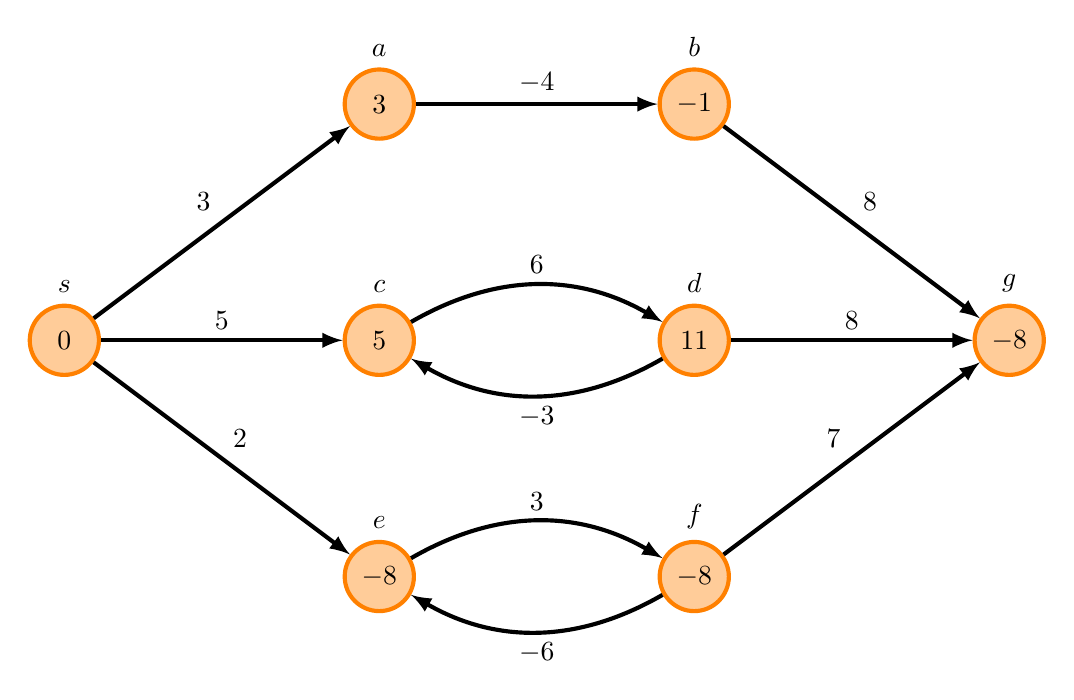
\begin{tikzpicture}[
    ->, 
    >=latex, % Use LaTeX-style arrows
    line width=1.5pt, % Increase the thickness of the arrow lines
    >=latex, scale=2, % Scale the arrowheads
    node distance=4cm and 0.2cm, % Adjust node distance (horizontal and vertical)
    auto % Automatically position labels
]

% Nodes with labels
\node[state,fill=orange!40,draw=orange ,label=above:{$\huge s$}] (A) {$0$};
\node[state,fill=orange!40,draw=orange , label=above:{$c$}] (B) [right of=A] {$5$};
\node[state,fill=orange!40,draw=orange , label=above:{$d$}] (C) [right of=B] {$11$};
\node[state,fill=orange!40,draw=orange , label=above:{$g$}] (D) [right of=C] {$-8$};

\node[state,fill=orange!40,draw=orange , label=above:{$a$}] (E) [above of=B,yshift=-1cm] {$3$};
\node[state, fill=orange!40,draw=orange ,label=above:{$b$}] (F) [above of=C,yshift=-1cm] {$-1$};

\node[state,fill=orange!40,draw=orange , label=above:{$e$}] (G) [below of=B,yshift=1cm] {$-8$};
\node[state, fill=orange!40,draw=orange ,label=above:{$f$}] (H) [below of=C,yshift=1cm] {$-8$};

% Edges with labels
\path (A) edge node {$5$} (B);
\path (B) edge[bend left] node {$6$} (C);
\path (C) edge[bend left] node {$-3$} (B);
\path (C) edge node {$8$} (D);

\path (A) edge node {$3$} (E);
\path (E) edge node {$-4$} (F);
\path (F) edge node {$8$} (D);

\path (A) edge node {$2$} (G);
\path (G) edge[bend left] node {$3$} (H);
\path (H) edge[bend left] node {$-6$} (G);
\path (H) edge node {$7$} (D);

\end{tikzpicture}

\section{Practice Graph 2(List)}
\vspace{50pt}
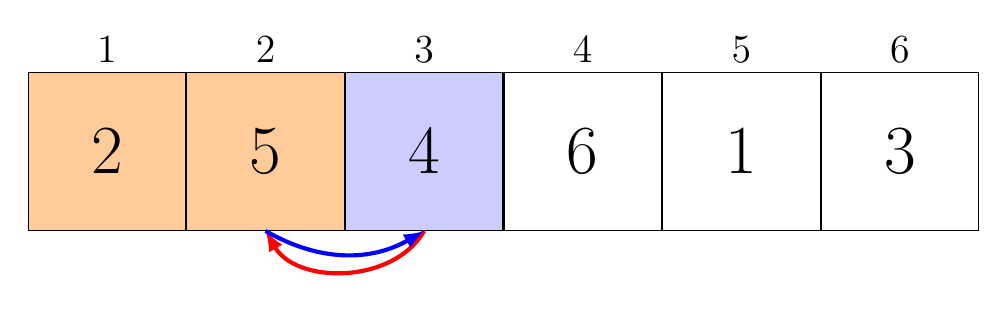
\begin{tikzpicture}[
    % Define a custom style for nodes
    mynode/.style={
        draw,
        rectangle,
        minimum width=2cm,
        minimum height=2cm
    }
]

% Define nodes using the custom style
\node[mynode,fill=orange!40,label=above:{\Large $1$}] (A) {\Huge 2};
\node[mynode, fill=orange!40,right=0pt of A,label=above:{\Large $2$}] (B) {\Huge 5};
\node[mynode,fill=blue!20, right=0pt of B,label=above:{\Large $3$}] (C) {\Huge 4};
\node[mynode, right=0pt of C,label=above:{\Large $4$}] (D) {\Huge 6};
\node[mynode, right=0pt of D,label=above:{\Large $5$}] (E) {\Huge 1};
\node[mynode, right=0pt of E,label=above:{\Large $6$}] (F) {\Huge 3};

% Edges with specific start and end points
\draw[red, line width=1.5pt, ->, >=latex, bend left=60] (C.south) to (B.south); % C to B with more bend
\draw[blue, line width=1.5pt, ->, >=latex,bend right=30] (B.south) to (C.south); % B to C with less bend

\end{tikzpicture}
\end{document}
